\documentclass[12pt]{article}

% import packages
\usepackage[utf8]{inputenc}
\usepackage{float}
\usepackage{subfloat}
\usepackage{subfig}
\usepackage{amsmath}
\usepackage[toc,page]{appendix}
\usepackage{caption}
\usepackage{graphicx}
\usepackage{hyperref}
\usepackage[left=1in,top=0.75in,right=1in,bottom=0.75in]{geometry}

\graphicspath{ {./images} }
% hyperref setup
\hypersetup{
	colorlinks=true,
	linkcolor=blue,
	filecolor=blue,      
	urlcolor=blue,
	citecolor=blue,
	pdftitle={IEP Design Project},
	pdfpagemode=FullScreen,
}

% titlepage	
\title{\textbf{IEP Design Project}}
\author{Callum Stephenson, css47}
\date{}

\begin{document}
    \begin{titlepage}
        \maketitle
        \thispagestyle{empty}
        \vspace{13cm}
        \textbf{Department of Engineering, University of Cambridge}
    \end{titlepage}
    \tableofcontents
    \newpage
    \section{Introduction}
        Modern electronic systems use micro electromechanical systems in order to detect motion. This motion tracking may be an added feature or vital to their function.
        The aim of this report is to build a circuit where the output of the accelerometer could be easily visualised using a set of LEDs varying on the output signal
        strength. The single axis of tilt is measured and the output displayed on a set of LEDs using op-amps set up as comparators in order to easily see the output level.
    \section{Circuit setup}
        The aim of this circuit is to have a tilt-sensing circuit from the kitset and a 5V USB phone charger.
        \subsection{Circuit diagram}
        \begin{figure}[H]
            \captionsetup{labelfont=bf}
            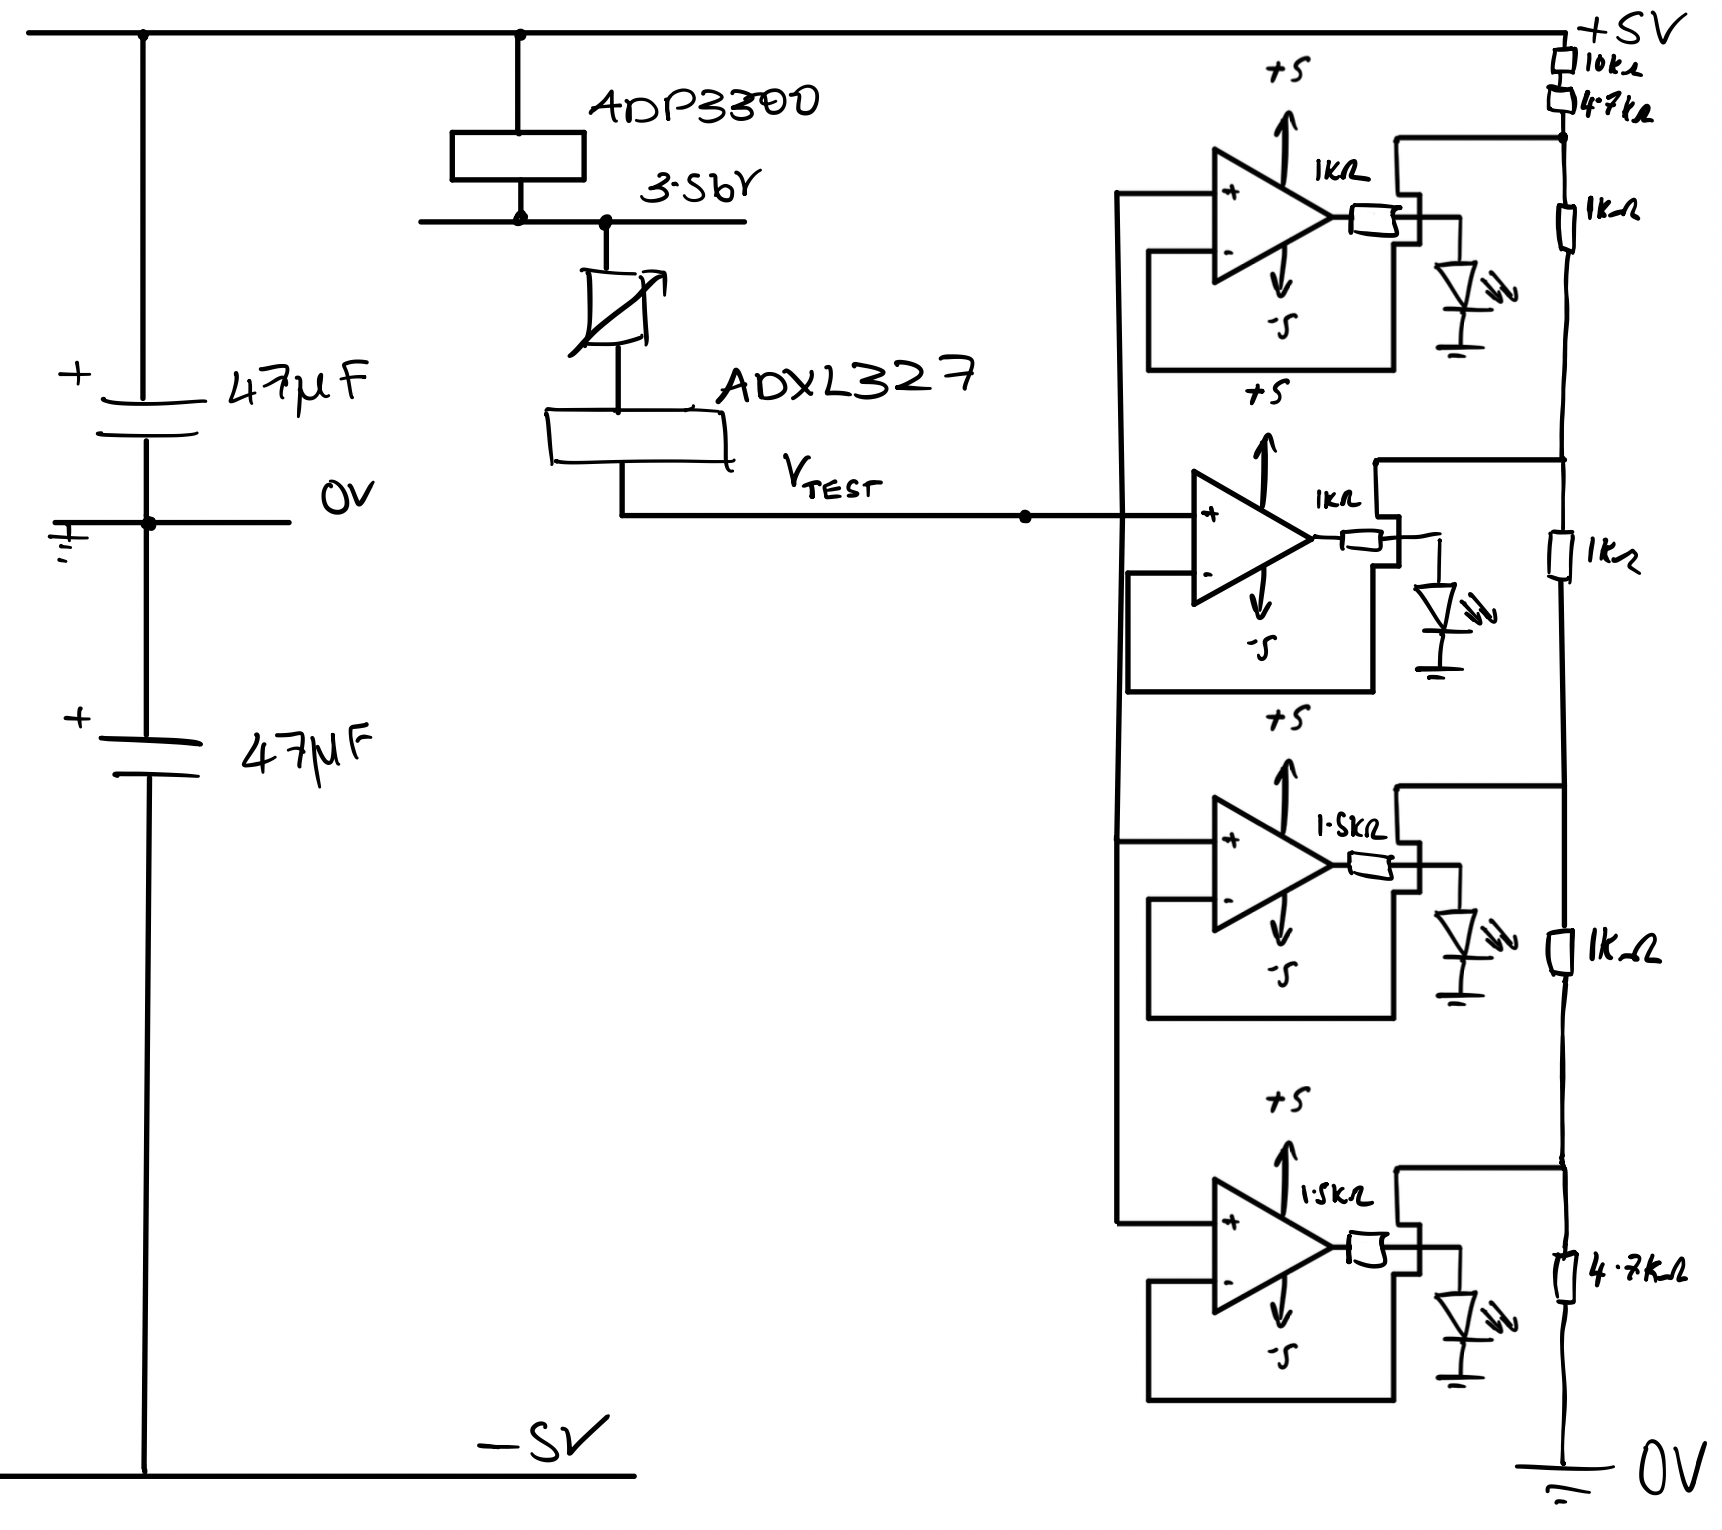
\includegraphics[width=30pc]{circuit_diagram.png}
            \caption{Circuit diagram showing the complete circuit}\label{figure1}
        \end{figure}
        \subsection{Component list}
            \begin{tabular}{ |c|c| }
                \hline
                Component & Quantity \\
                \hline
                LED & 4 \\
                \hline
                1 k$\Omega$ & 4 \\
                \hline
                1.5 k$\Omega$ & 3 \\
                \hline
                10 k$\Omega$ & 1 \\
                \hline
                4.7 k$\Omega$ & 2 \\
                \hline
                OP27 & 2 \\
                \hline
                OP37 & 2 \\
                \hline
                Breadboard & 1 \\
                \hline
                USB daughter board & 1 \\
                \hline
                47 $\mu$F capacitor & 2 \\
                \hline
                LTM8067Y converter & 1 \\
                \hline
                5 k$\Omega$ potentiometer & 1 \\
                \hline
                ADP3300 regulator & 1 \\
                \hline
                ADXL327 accelerometer & 1 \\
                \hline
            \end{tabular}
        \subsection{Design process}
            Each part of functional area of the circuit was considered separately in order to cater to the needs of the sensing and LED circuit.
            \subsubsection{Supply of power}
                We were able to use the micro usb daughter board in conjunction with the LTM8067Y in order to get a bipolar $\pm$5 V supply rail. This
                was required in order to have proper power supply to the OP27 and OP37 operational amplifiers. Two capacitors were connected to the output
                of the LTM8067Y chip in order to reduce noise within the circuit. \\ \\
                The ADP3300 was used in order to provide a suitable voltage to the accelerometer, which should be around 3.3V in theory, however during measurement
                a voltage of 3.56V was observed. To reduce this down to below 3.3V the potentiometer was connected to the output to ensure the output voltage was
                less than 3.3V. 
            \subsubsection{Accelerometer output}
            To be able to have a set of op-amps working as comparators to visualise the output of the accelerometer, the output must first be checked. From testing
            we found that the x channel had the biggest voltage swing and thus would be the easiest to bias given the standard set of resistors available. \\ \\
            \begin{tabular}{ |c|c|c|c| }
                \hline
                Initial angle & Final angle & Start voltage (V) & End voltage (V) \\
                \hline
                0 & 45 & 1.4 & 1.17 \\
                \hline
                45 & 90 & 1.17 & 1.05 \\
                \hline
                -45 & 0 & 1.7 & 1.4 \\
                \hline
            \end{tabular}
            \subsubsection{Operational amplifer testing}
                Testing one op-amp will give information about function which can be used to design the rest of the circuit. The x channel of the ADXL327 was connected
                to the positive $In_+$ of the op-amp. The reference voltage was around 1.6V, and from this the potential divider equation could be used to obtain a ratio between
                $R_1$ and $R_2$. 
                \begin{equation}
                    \frac{R_2}{R_1+R_2}.5 = 1.6 \\
                    \frac{R_1+R_2}{R_2} = 0.32 \\
                \end{equation}
                Hence sensible values to try would be around $R_1$ = 2.2 k$\Omega$ and $R_2$ = 1 k$\Omega$. Using these values the op-amp changed from 4.5 V to 0.5 V when the
                required angle of tilt was reached. A resistor was connected in series with the output LED in order to protect the LED from voltage overload. 
            \subsubsection{Voltage comparators}
            A sequence of series resistors is the easiest way to get the required voltage to test against $V_{test}$, and we should set the voltage inbetween the resistors
            to be close to significant values in the tilt. Based on the measurement in prior sections; reference voltages of 1.4 V, 1.17 V, 1.05 V, 1.7 V.
            Using five resistors in series was able to give values close to the reference voltages. $R_2$, $R_3$, $R_4$ were each set at 1 k$\Omega$. Plugging that in to the
            potential divider equation, that yields $R_5$ = 4.7 k$\Omega$, and $R_1$ = 14.9 k$\Omega$. \\
            Measuring the voltages produced by using the closest approximate standard components to this setup yielded results of: 1.7V, 1.54V, 1.27V , 1.04V. These are relatively
            close to the reference values and such should be suitable for using with the 4 op-amp comparators. \\
            This means that each op-amp can be connected to the connection between the two LEDs, and different values of tilt can be visualised with the LEDs.
    \subsection{Observations}
            When the USB power source was connected to the circuit, the first LED came on. When tilted the second and third LEDs came on. Initially there were some
            issues trying to get the LEDs to turn on, and adjusting the offset did not help. We tried to use an op-amp difference amplifier to fix this but this
            still resulted in undesirable behaviour. We managed to get it to work partially by holding the board against a surface and holding the accelerometer whilst tilting.
            Hence the bad video, as one hand was needed to hold and the other to tilt, so the phone was on a slightly elevated postiion on the desk. 
    \subsection{Conclusion \& limitations}
    Overall the function displayed in the end is as expected, minus some jitter from the ADP3300 regulator. The signal from the ADXL327 also flickered a lot. It was a combination
    of both of these that caused the LEDs to flicker whilst moving the breadboard. One limitation is that only one axis is visuaslied. If there were more LEDs and op-amps
    then it would be possible to visualise both the z and y axis too. One idea would be to have the signal to a digital output, but there is nothing that is capable of doing
    this within the kitset. One use for the output if it was able to be measured in 3 axis would be a game controller, which would be interesting to implement. \\ \\
    A different circuit setup may have produced more desirable and consistent results, so in the future if rebuilding were necessary it might be worthwhile to explore different
    avenues of amplification and display of the signal strength. Given the limitations of the kitset, the performance was adequate. Given more resistor values, it would be
    easier to get exactly the right reference values which would make the tilt sensing closer to 45/90/0 providing more accurate visualisation of the output.
\end{document}